\chapter{Занятие 1. Случайные события.}


\section*{Введение}

Задачи, с которыми сталкивается человек в окружающем мире, сформулированы на естественном языке. Первым этапом решения задачи является формализация --- формулировка задачи
с помощью математических объектов некоторой формальной схемы. В теории вероятностей такой схемой является \textbf{вероятностное пространство} $\left ( \Omega, \Sigma, P \right )$,
в котором:
\begin{enumerate}
    \item $\Omega$ --- множество элементарных исходов,
    \item $\Sigma$ --- алгебра событий,
    \item $P$ --- вероятностная мера.
\end{enumerate}

\section*{Задача 18.1}

Игральная кость подбрасывается дважды. Наблюдаемый результат --- пара чисел, соответствующих числам очков, выпавших в первый и второй раз. События
\begin{itemize}
    \item $A = \event{\text{оба раза выпало число очков кратное трём}}$,
    \item $B = \event{\text{ни разу не выпало число шесть}}$,
    \item $C = \event{\text{оба раза выпало число очков, большее трех}}$,
    \item $D = \event{\text{оба раза выпало одинаковое число очков}}$.
\end{itemize}
Необходимо построить множество элементарных исходов $\Omega$ и подмножества, соответствующие событиям $A$ -- $D$.

\subsection*{Решение}

\begin{enumerate}
    \item
    Каждый элементарный исход можно преставить парой чисел $(i, j)$, где $i$ обозначает количество очков, выпавших в первый рах, а $j$ --- во второй, тогда множество всех элементарных
    исходов:
    \begin{equation}
        \Omega = \set{(i, j) : i, j \in \set{1, 2, 3, 4, 5, 6}}.
    \end{equation}

    Множество всех элементарных исходов удобно представить в виде таблицы:
    \begin{center}
        \begin{tabular}{c|c|c|c|c|c|c|}
            $i$, $j$ & 1         & 2         & 3         & 4         & 5         & 6         \\
            \hline
            1        & $\bullet$ & $\bullet$ & $\bullet$ & $\bullet$ & $\bullet$ & $\bullet$ \\
            \hline
            2        & $\bullet$ & $\bullet$ & $\bullet$ & $\bullet$ & $\bullet$ & $\bullet$ \\
            \hline
            3        & $\bullet$ & $\bullet$ & $\bullet$ & $\bullet$ & $\bullet$ & $\bullet$ \\
            \hline
            4        & $\bullet$ & $\bullet$ & $\bullet$ & $\bullet$ & $\bullet$ & $\bullet$ \\
            \hline
            5        & $\bullet$ & $\bullet$ & $\bullet$ & $\bullet$ & $\bullet$ & $\bullet$ \\
            \hline
            6        & $\bullet$ & $\bullet$ & $\bullet$ & $\bullet$ & $\bullet$ & $\bullet$ \\
            \hline
        \end{tabular}
    \end{center}

    \item
    Событие $A$ состоит из следующих элементарных исходов:
    \begin{equation}
        A = \set{(3,3), (3,6), (6,3), (6,6)} .
    \end{equation}
    В виде таблицы:
    \begin{center}
        \begin{tabular}{c|c|c|c|c|c|c|}
            $i$, $j$ & 1 & 2 & 3         & 4 & 5 & 6         \\
            \hline
            1        &   &   &           &   &   &           \\
            \hline
            2        &   &   &           &   &   &           \\
            \hline
            3        &   &   & $\bullet$ &   &   & $\bullet$ \\
            \hline
            4        &   &   &           &   &   &           \\
            \hline
            5        &   &   &           &   &   &           \\
            \hline
            6        &   &   & $\bullet$ &   &   & $\bullet$ \\
            \hline
        \end{tabular}
    \end{center}

    \item
    Событие $B$ состоит из следующих элементарных исходов:
    \begin{multline}
        B = \left \{ (1,1), (1,2), (1,3), (1,4), (1,5), \right . \\
        (2,1), (2,2), (2,3), (2,4), (2,5), \\
        (3,1), (3,2), (3,3), (3,4), (3,5), \\
        (4,1), (4,2), (4,3), (4,4), (4,5), \\
        \left . (5,1), (5,2), (5,3), (5,4), (5,5) \right \} .
    \end{multline}
    В виде таблицы:
    \begin{center}
        \begin{tabular}{c|c|c|c|c|c|c|}
            $i$, $j$ & 1         & 2         & 3         & 4         & 5         & 6 \\
            \hline
            1        & $\bullet$ & $\bullet$ & $\bullet$ & $\bullet$ & $\bullet$ &   \\
            \hline
            2        & $\bullet$ & $\bullet$ & $\bullet$ & $\bullet$ & $\bullet$ &   \\
            \hline
            3        & $\bullet$ & $\bullet$ & $\bullet$ & $\bullet$ & $\bullet$ &   \\
            \hline
            4        & $\bullet$ & $\bullet$ & $\bullet$ & $\bullet$ & $\bullet$ &   \\
            \hline
            5        & $\bullet$ & $\bullet$ & $\bullet$ & $\bullet$ & $\bullet$ &   \\
            \hline
            6        &           &           &           &           &           &   \\
            \hline
        \end{tabular}
    \end{center}

    \item
    Событие $C$ состоит из следующих элементарных исходов:
    \begin{equation}
        C = \set{(4,4), (4,5), (4,6), (5,4), (5,5), (5,6), (6,4), (6,5), (6,6)} .
    \end{equation}
    В виде таблицы:
    \begin{center}
        \begin{tabular}{c|c|c|c|c|c|c|}
            $i$, $j$ & 1 & 2 & 3 & 4         & 5         & 6         \\
            \hline
            1        &   &   &   &           &           &           \\
            \hline
            2        &   &   &   &           &           &           \\
            \hline
            3        &   &   &   &           &           &           \\
            \hline
            4        &   &   &   & $\bullet$ & $\bullet$ & $\bullet$ \\
            \hline
            5        &   &   &   & $\bullet$ & $\bullet$ & $\bullet$ \\
            \hline
            6        &   &   &   & $\bullet$ & $\bullet$ & $\bullet$ \\
            \hline
        \end{tabular}
    \end{center}

    \item
    Событие $D$ состоит из следующих элементарных исходов:
    \begin{equation}
        D = \set{(1,1), (2,2), (3,3), (4,4), (5,5), (6,6)} .
    \end{equation}
    В виде таблицы:
    \begin{center}
        \begin{tabular}{c|c|c|c|c|c|c|}
            $i$, $j$ & 1         & 2         & 3         & 4         & 5         & 6         \\
            \hline
            1        & $\bullet$ &           &           &           &           &           \\
            \hline
            2        &           & $\bullet$ &           &           &           &           \\
            \hline
            3        &           &           & $\bullet$ &           &           &           \\
            \hline
            4        &           &           &           & $\bullet$ &           &           \\
            \hline
            5        &           &           &           &           & $\bullet$ &           \\
            \hline
            6        &           &           &           &           &           & $\bullet$ \\
            \hline
        \end{tabular}
    \end{center}
\end{enumerate}

\subsection*{Ответ:}
\begin{enumerate}
    \item $\Omega = \set{(i, j) : i, j \in \set{1, 2, 3, 4, 5, 6}}$,
    \item $A = \set{(i, j) : i, j \in \set{3, 6}}$,
    \item $B = \set{(i, j) : i, j \in \set{1, 2, 3, 4, 5}}$,
    \item $C = \set{(i, j) : i, j \in \set{4, 5, 6}}$,
    \item $D = \set{(i, i) : i \in \set{1, 2, 3, 4, 5, 6}}$.
\end{enumerate}

\section*{Задача 18.3}

Монета подбрасывается до первого появления герба. Наблюдаемый результат --- общее число подбрасываний. События:
\begin{enumerate}
    \item $A = \event{\text{герб выпал при третьем подбрасывании}}$,
    \item $B = \event{\text{герб выпал не ранее, чем при третьем подбрасывании}}$.
\end{enumerate}
Построить множество элементарных исходов $\Omega$ и подмножества, соответствующие событиям $A$ и $B$.

\subsection*{Решение}

Элементарные исходы представим в виде конечного набора решек ("Р"), которые заканчиваются гербом ("Г"):
\begin{align*}
    \omega_1 = & \left ( \text{Г} \right ) , \\
    \omega_2 = & \left ( \text{Р}, \text{Г} \right ) , \\
    \omega_3 = & \left ( \text{Р}, \text{Р}, \text{Г} \right ) , \\
    \omega_4 = & \left ( \text{Р}, \text{Р}, \text{Р}, \text{Г} \right ) , \\
    & \dots \\
    \omega_n = & \left ( \overbrace{\text{Р}, \dots, \text{Р}}^{n-1}, \text{Г} \right ), \\
    & \dots
\end{align*}
Множество всех элеметарных исходов $\Omega = \set{\omega_1, \omega_2, \omega_3, \omega_4, \dots }$. В данном случае множество $\Omega$ является счетным.

Событие $A = \set{\omega_3}$, событие $B = \set{\omega_i : 3 \le i}$.

\subsection*{Ответ:}
Элементарный исход $\omega_n$ обозначает выпадение герба на $n$-ом подбрасывании.
\begin{enumerate}
    \item $\Omega = \set{\omega_n: n \in \mathbb{N}}$,
    \item $A = \set{\omega_3}$,
    \item $B = \set{\omega_i: 3 \le i}$.
\end{enumerate}


\section{Задача 18.5}

Производится стрельба по плоской прямоугольной мишени: $-2 \le x \le 2$, $-1 \le y \le 1$. Наблюдаемый результат --- координаты точки попадания в декартовой системе координат.
По условиям стрельбы непопадание в указанный прямоугольник исключено. События:
\begin{enumerate}
    \item $A = \event{\text{абсцисса точки попадания не меньше ординаты}}$,
    \item $B = \event{\text{произведение координат точки неотрицательно}}$,
    \item $C = \event{\text{сумма абсолютных величин координат точки превышает единицу}}$.
\end{enumerate}
Построить множество элементарных исходов $\Omega$ и подмножества, соответствующие событиям. Выявить пары совместных событий.

\subsection*{Решение:}

Элементарным исходом является пара координат $\left ( x, y \right )$, где $-2 \le x \le 2$ и $-1 \le y \le 1$. Множество элементарных исходов $\Omega$ --- прямоугольник:
\begin{equation}
    \Omega = \set{(x, y): -2 \le x \le 2, -1 \le y \le 1}.
\end{equation}

\begin{figure}[h]
    \centering
    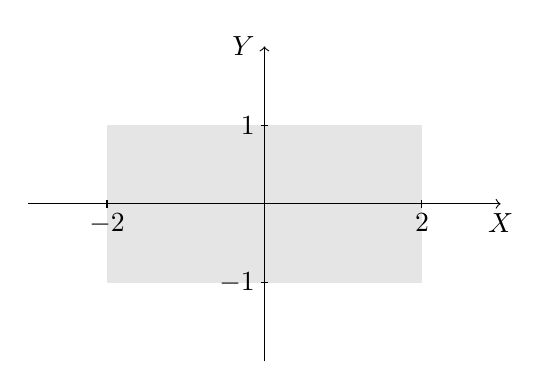
\begin{tikzpicture}
        % множество
        \path [fill=gray!20] ( -2, -1 ) rectangle ( 2, 1 );

        % оси
        \draw [->] ( -3, 0 ) -- ( 3, 0 ) node [below] at ( 3, 0 ) {$X$};
        \draw [->] ( 0, -2 ) -- ( 0, 2 ) node [left] at ( 0, 2 ) {$Y$};

        % отметки
        \draw ( 2, -0.05 ) -- ( 2, 0.05 ) node [below] at ( 2, 0 ) {$2$};
        \draw ( -2, -0.05 ) -- ( -2, 0.05 ) node [below] at ( -2, 0 ) {$-2$};
        \draw ( -0.05, 1 ) -- ( 0.05, 1 ) node [left] at ( 0, 1 ) {$1$};
        \draw ( -0.05, -1 ) -- ( 0.05, -1 ) node [left] at ( 0, -1 ) {$-1$};
    \end{tikzpicture}
    \caption{Множество элементаных исходов $\Omega$.}
\end{figure}

События:
\begin{enumerate}
    \item $A = \set{(x, y): x \ge y}$,
    \item $B = \set{(x, y): x \cdot y \ge 0}$,
    \item $C = \set{(x, y): \modulus{x} + \modulus{y} > 1}$.
\end{enumerate}

Совместными являются события, которые могут наступить одновременно, то есть события, у которых есть общие элементарные исходны. Пары совместных событий: $A$ и $B$, $A$ и $C$,
$B$ и $C$.

\begin{figure}[h]
    \centering
    \begin{subfigure}{0.3\textwidth}
        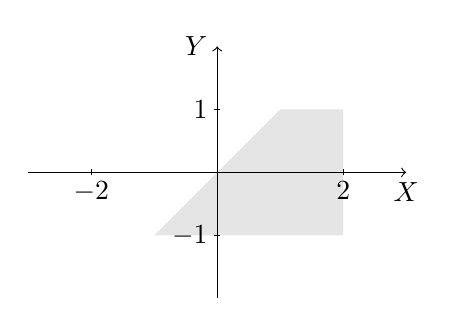
\begin{tikzpicture}[scale=0.8]
            % множество
            \path [fill=gray!20] ( -1, -1 ) -- ( 1, 1 ) -- ( 2, 1 ) -- ( 2, -1 ) -- ( -1, -1 );
            % оси
            \draw [->] ( -3, 0 ) -- ( 3, 0 ) node [below] at ( 3, 0 ) {$X$};
            \draw [->] ( 0, -2 ) -- ( 0, 2 ) node [left] at ( 0, 2 ) {$Y$};

            % отметки
            \draw ( 2, -0.05 ) -- ( 2, 0.05 ) node [below] at ( 2, 0 ) {$2$};
            \draw ( -2, -0.05 ) -- ( -2, 0.05 ) node [below] at ( -2, 0 ) {$-2$};
            \draw ( -0.05, 1 ) -- ( 0.05, 1 ) node [left] at ( 0, 1 ) {$1$};
            \draw ( -0.05, -1 ) -- ( 0.05, -1 ) node [left] at ( 0, -1 ) {$-1$};
        \end{tikzpicture}
        \caption{Событие $A$}
    \end{subfigure}
    \hfill
    \begin{subfigure}{0.3\textwidth}
        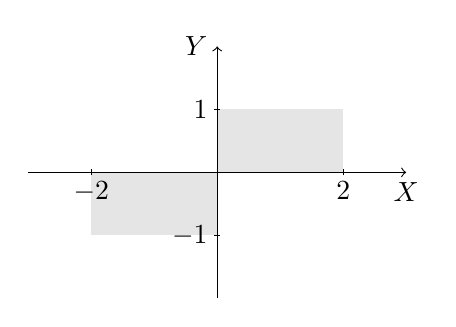
\begin{tikzpicture}[scale=0.8]
            % множество
            \path [fill=gray!20] ( -2, -1 ) rectangle ( 0, 0 );
            \path [fill=gray!20] ( 0, 0 ) rectangle ( 2, 1 );

            % оси
            \draw [->] ( -3, 0 ) -- ( 3, 0 ) node [below] at ( 3, 0 ) {$X$};
            \draw [->] ( 0, -2 ) -- ( 0, 2 ) node [left] at ( 0, 2 ) {$Y$};

            % отметки
            \draw ( 2, -0.05 ) -- ( 2, 0.05 ) node [below] at ( 2, 0 ) {$2$};
            \draw ( -2, -0.05 ) -- ( -2, 0.05 ) node [below] at ( -2, 0 ) {$-2$};
            \draw ( -0.05, 1 ) -- ( 0.05, 1 ) node [left] at ( 0, 1 ) {$1$};
            \draw ( -0.05, -1 ) -- ( 0.05, -1 ) node [left] at ( 0, -1 ) {$-1$};
        \end{tikzpicture}
        \caption{Событие $B$}
    \end{subfigure}
    \hfill
    \begin{subfigure}{0.3\textwidth}
        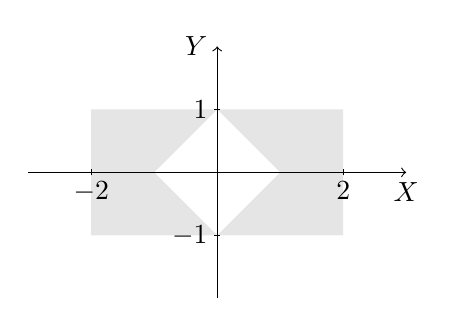
\begin{tikzpicture}[scale=0.8]
            % множество
            \path [fill=gray!20] ( 0, 1 ) -- ( 2, 1 ) -- ( 2, 0 ) -- ( 1, 0 );
            \path [fill=gray!20] ( 0, 1 ) -- ( -2, 1 ) -- ( -2, 0 ) -- ( -1, 0 );
            \path [fill=gray!20] ( 0, -1 ) -- ( 2, -1 ) -- ( 2, 0 ) -- ( 1, 0 );
            \path [fill=gray!20] ( 0, -1 ) -- ( -2, -1 ) -- ( -2, 0 ) -- ( -1, 0 );

            % оси
            \draw [->] ( -3, 0 ) -- ( 3, 0 ) node [below] at ( 3, 0 ) {$X$};
            \draw [->] ( 0, -2 ) -- ( 0, 2 ) node [left] at ( 0, 2 ) {$Y$};

            % отметки
            \draw ( 2, -0.05 ) -- ( 2, 0.05 ) node [below] at ( 2, 0 ) {$2$};
            \draw ( -2, -0.05 ) -- ( -2, 0.05 ) node [below] at ( -2, 0 ) {$-2$};
            \draw ( -0.05, 1 ) -- ( 0.05, 1 ) node [left] at ( 0, 1 ) {$1$};
            \draw ( -0.05, -1 ) -- ( 0.05, -1 ) node [left] at ( 0, -1 ) {$-1$};
        \end{tikzpicture}
        \caption{Событие $C$}
    \end{subfigure}
    \caption{События $A$, $B$, $C$.}
\end{figure}

\subsection*{Ответ:}
\begin{enumerate}
    \item Множество всех элементарных исходов $\Omega = \set{(x, y): -2 \le x \le 2, -1 \le y \le 1}$.
    \item $A = \set{(x, y): x \ge y}$.
    \item $B = \set{(x, y): x \cdot y \ge 0}$.
    \item $C = \set{(x, y): \modulus{x} + \modulus{y} > 1}$.
    \item Пары совместных событий: $A$ и $B$, $A$ и $C$, $B$ и $C$.
\end{enumerate}

